\documentclass{article}

\usepackage{tikz}
 
\begin{document}

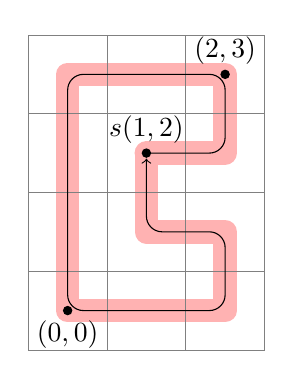
\begin{tikzpicture}
	\draw[line width=0.3cm,color=red!30,cap=round,join=round] 
		(1.5, 2.5)-- ++(1, 0) -- ++(0, 1) -- ++(-1, 0) -- ++(-1, 0) -- ++(0, -1) -- ++(0, -1)
		-- ++(0, -1) --++ (1, 0) --++ (1, 0) --++ (0, 1) --++ (-1, 0) --++ (0, 1);
		
	\draw[help lines] (0, 0) grid (3, 4);
	\draw[above] (1.5,2.5) node(s){$s(1, 2)$};
	\draw[below] (0.5,0.5) node(s){$(0, 0)$};
	\draw[above] (2.5,3.5) node(s){$(2, 3)$};
	\fill (1.5,2.5) circle (0.06cm) (0.5,0.5) circle (0.06cm) (2.5, 3.5) circle (0.06cm);
	
  	\draw[->,rounded corners=0.2cm,shorten >=2pt]
  	(1.5, 2.5)-- ++(1, 0) -- ++(0, 1) -- ++(-1, 0) -- ++(-1, 0) -- ++(0, -1) -- ++(0, -1)
  	-- ++(0, -1) --++ (1, 0) --++ (1, 0) --++ (0, 1) --++ (-1, 0) --++ (0, 1);
\end{tikzpicture}

\end{document}